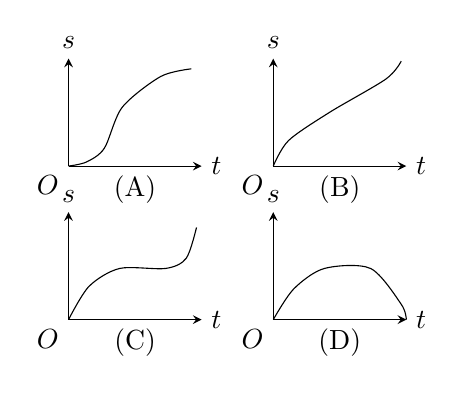
\begin{tikzpicture}[>=stealth,scale=.65]
\foreach \x/\y/\lab in {0/0/A,4/0/B,0/-3/C,4/-3/D}{
  \begin{scope}[shift={(\x,\y)}]
    \draw[->] (0,0)--(2.6,0) node[right] {$t$};
    \draw[->] (0,0)--(0,2.1) node[above] {$s$};
    \node[below left] at (0,0) {$O$};
    \node at (1.3,-.45) {(\lab)};
  \end{scope}
}
\draw plot[smooth] coordinates {(0,0) (.35,.08) (.7,.35) (1.05,1.15) (1.8,1.75) (2.4,1.9)};
\draw[shift={(4,0)}] plot[smooth] coordinates {(0,0) (.3,.5) (1.1,1.05) (2.2,1.7) (2.5,2.05)};
\draw[shift={(0,-3)}] plot[smooth] coordinates {(0,0) (.4,.65) (1.0,1.0) (1.9,1.0) (2.3,1.2) (2.5,1.8)};
\draw[shift={(4,-3)}] plot[smooth] coordinates {(0,0) (.4,.6) (1.0,1.0) (1.9,1.0) (2.5,.3) (2.6,0)};
\end{tikzpicture}
